%!TEX root = /Users/louis/Documents/PhD/Deliverables/Thesis/thesis.tex

\section{Transformation Tools Contest}
The Transformation Tools Contest (TTC) is a workshop series that seeks to compare and contrast tools for performing model and graph transformation. At TTC 2010, two rounds of submissions were invited: cases (transformation problems, three of which are selected by the workshop organisers) and solutions to the selected cases. In addition, TTC 2010 include a \emph{live contest}: during the workshop a further transformation problem was announced and solutions submitted.

Participation in TTC 2010 facilitated further evaluation of Flock. Flock and 8 other transformation tools were assessed for a model migration problem based on a real-world example of metamodel evolution from the UML \cite{uml22}. As part of the live contest, Flock was also assessed along with 13 transformation tools for a model transformation problem. Compared to the evaluation described in Section~\ref{subsec:collaborative_comparison}, the evaluation in this section compares Flock to a wider range of tools (model and graph transformation tools, and not just model migration tools), and investigates the suitability of Flock for specifying model transformation.

The remainder of this section describes the model migration problem (Section~\ref{subsubsec:ttc_case}) and Flock solution (Section~\ref{subsubsec:ttc_solution}), and the use of Flock for specifying a model transformation in the live contest (Section~\ref{subsubsec:ttc_live_contest}).

\subsection{Model Migration Case}
\label{subsubsec:ttc_case}
To compare Flock with other transformation tools for specifying model migration, the thesis author submitted a case to TTC based on the evolution of the UML. The way in which activity diagrams are modelled in the UML changed significantly between versions 1.4 and 2.1 of the specification. In the former, activities were defined as a special case of state machines, while in the latter they are defined atop a more general semantic base\footnote{A variant of generalised coloured Petri nets.} \cite{selic05uml2}.

The remainder of this section briefly introduces UML activity diagrams, describes their evolution, and discusses the way in which solutions were assessed. The work presented in this section is based on the case submitted to TTC 2010 \cite{rose10ttc_case}. 

\subsubsection{Activity Diagrams in UML}
Activity diagrams are used for modelling lower-level behaviours, emphasising sequencing and co-ordination conditions. They are used to model business processes and logic \cite{uml22}. Figure~\ref{fig:activity} shows an activity diagram for filling orders. The diagrams is partitioned into three \emph{swimlanes}, representing different organisational units. \emph{Activities} are represented with rounded rectangles and \emph{transitions} with directed arrows. \emph{Fork} and \emph{join} nodes are specified using a solid black rectangle. \emph{Decision} nodes are represented with a diamond. Guards on transitions are specified using square brackets. For example, in Figure~\ref{fig:activity} the transition to the restock activity is guarded by the condition \texttt{[not in stock]}. Text on transitions that is not enclosed in square brackets represents a trigger event. In Figure~\ref{fig:activity}, the transition from the restock activity occurs on receipt of the asynchronous signal called \texttt{receive stock}. Finally, the transitions between activities might involve interaction with objects. In Figure~\ref{fig:activity}, the Fill Order activity leads to an interaction with an object called \texttt{Filled Object}. 

\begin{figure}[htbp]
  \centering
  \includegraphics*[viewport=75 230 585 800,width=13cm]{6.Evaluation/images/activity.pdf}
  \caption{Activity model to be migrated.}
  \label{fig:activity}
\end{figure}

Between versions 1.4 and 2.2 of the UML specification, the metamodel for activity diagrams has changed significantly. The sequel summarises most of the changes, and details can be found in \cite{uml14} and \cite{uml22}.

\subsubsection{Evolution of Activity Diagrams}
Figures~\ref{fig:uml14} and \ref{fig:uml22} are simplifications of the activity diagram metamodels from versions 1.4 and 2.2 of the UML specification, respectively. In the interest of clarity, some features and abstract classes have been removed from Figures~\ref{fig:uml14} and \ref{fig:uml22}.

Some differences between Figures~\ref{fig:uml14} and \ref{fig:uml22} are: activities have been changed such that they comprise nodes and edges, actions replace states in UML 2.2, and the subtypes of control node replace pseudostates.

\begin{figure}[htbp]
  \centering
  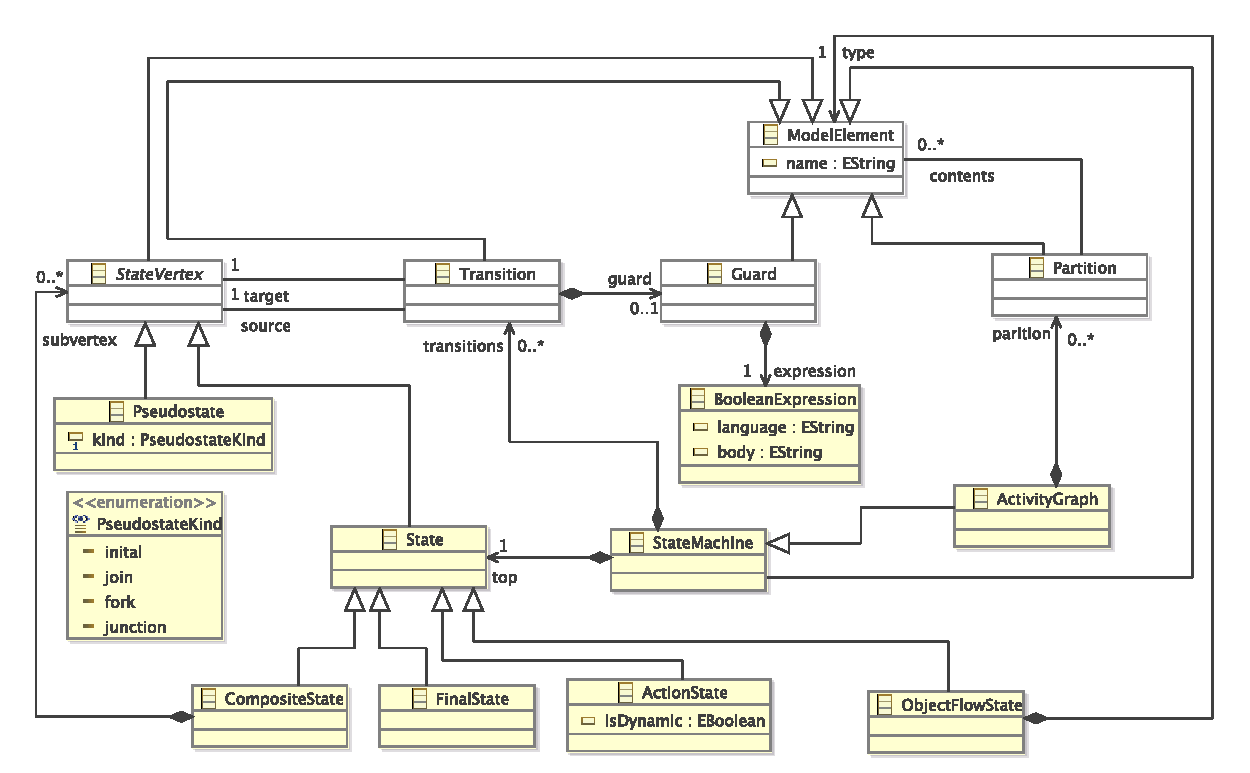
\includegraphics[width=12cm]{6.Evaluation/images/uml14.pdf}
  \caption{UML 1.4 Activity Graphs (based on \cite{uml14}).}
  \label{fig:uml14}
\end{figure}
 

\begin{figure}[htbp]
  \centering
  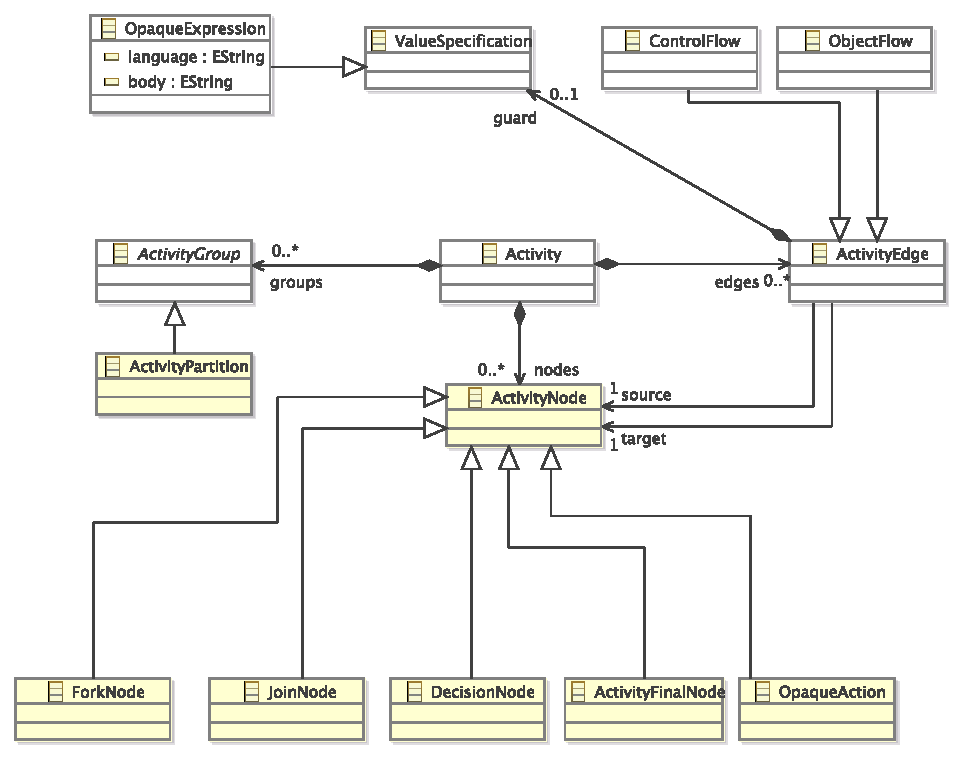
\includegraphics[width=12cm]{6.Evaluation/images/uml22.pdf}
  \caption{UML 2.2 Activity Diagrams (based on \cite{uml22}).}
  \label{fig:uml22}
\end{figure}

To facilitate the comparison of solutions, the exemplar model shown in Figure~\ref{fig:activity} was used. Figure~\ref{fig:activity} is based on \cite[pg3-165]{uml14}. Solutions migrated the activity diagram shown in Figure~\ref{fig:activity} -- which conforms to UML 1.4 -- to conform to UML 2.2. The UML 1.4 model, the migrated UML 2.2 model, and the UML 1.4 and 2.2 metamodels are available from\footnote{\url{http://www.cs.york.ac.uk/~louis/ttc/}}.

Submissions were evaluated using the following four criteria, which were decided by the thesis author and the workshop organisers:

\begin{itemize}
	\item \textbf{Correctness}: Does the transformation produce a model equivalent to the migrated UML 2.2. model included in the case resources?
	\item \textbf{Conciseness}: How much code is required to specify the transformation? (In \cite{sprinkle04domain} et al. propose that the amount of effort required to codify migration should be directly proportional to the number of changes between original and evolved metamodel).
		\item \textbf{Clarity}: How easy is it to read and understand the transformation? (For example, is a well-known or standardised language?)
		\item \textbf{Extensions}: Which of the case extensions (described below) were implemented in the solution?
\end{itemize}

To further distinguish between solutions, three extensions to the core task were proposed. The first extension was added after the case was submitted, and was proposed by the workshop organisers and the solution authors. The second and third extension were included in the case by the thesis author. 

\subsubsection{Extension 1: Alternative Object Flow State Migration Semantics}
\label{sub:object_flow_states}
Following the submission of the case, discussion on the TTC forums\footnote{\url{http://planet-research20.org/ttc2010/index.php?option=com_community&view=groups&task=viewgroup&groupid=4&Itemid=150} (registration required)} revealed an ambiguity in the UML 2.2 specification indicating that the migration semantics for the ObjectFlowState UML 1.4 concept are not clear from the UML 2.2 specification.

\textbf{In the core task} described above, instances of ObjectFlowState were migrated to instances of ObjectNode. Any instances of Transition that had an ObjectFlowState as their source or target were migrated to instances of ObjectFlow. Listing~\ref{lst:ofs_to_node} shows an example application of this migration semantics. The top line of Listing~\ref{lst:ofs_to_node} shows instances of UML 1.4 metaclasses, include an instance of ObjectFlowState. The bottom line of Listing~\ref{lst:ofs_to_node} shows the equivalent UML 2.2 instances according to this migration semantics. Note that the Transitions, t1 and t2, are migrated to an instance of ObjectFlow. Likewise, the instance of ObjectFlowState, s2, is migrated to an instance of ObjectFlow.

\begin{lstlisting}[caption=Migrating Actions, label=lst:ofs_to_node]
s1:State <- t1:Transition -> s2:ObjectFlowState <- t2:Transition -> s3:State

s1:ActivityNode <- t1:ObjectFlow -> s2:ObjectNode <- t2:ObjectFlow -> s3:ActivityNode
\end{lstlisting}

\textbf{This extension} considered an alternative migration semantics for ObjectFlowState. For this extension, instances of ObjectFlowState (and any connected Transitions) were migrated to instances ObjectFlow, as shown by the example in Listing~\ref{lst:ofs_to_flow} in which the UML 2.2 ObjectFlow, f1, replaces t1, t2 and s2.

\begin{lstlisting}[caption=Migrating Actions, label=lst:ofs_to_flow]
s1:State <- t1:Transition -> s2:ObjectFlowState <- t2:Transition -> s3:State

s1:ActivityNode <- f1:ObjectFlow -> s3:ActivityNode
\end{lstlisting}

The alternative semantics were proposed on the TTC 2010 forums, and agreed as an extension to the core task by consensus between the solution authors and the workshop organisers. 

\subsubsection{Extension 2: Concrete Syntax}
\label{sub:concrete_syntax}
The second extension relates to the appearance of activity diagrams. The UML specifications provide no formally defined metamodel for the concrete syntax of UML diagrams. However, some UML tools store diagrammatic information in a structured manner using XML or a modelling tool. For example, the Eclipse UML 2 tools \cite{mdt_uml2} store diagrams as GMF \cite{gronback09emp} diagram models.

As such, submissions were invited to explore the feasibility of migrating the concrete syntax of the activity diagram shown in Figure~\ref{fig:activity} to the concrete syntax in their chosen UML 2 tool. To facilitate this, the case resources included an ArgoUML project\footnote{\url{http://argouml.tigris.org/}} containing the activity diagram shown in Figure~\ref{fig:activity}.

\subsubsection{Extension 3: XMI}
\label{sub:xmi}
The UML specifications indicate that UML models should be stored using XMI. However, because XMI has evolved at the same time as UML, UML 1.4 tools most likely produce XMI of a different version to UML 2.2 tools. For instance, ArgoUML produces XMI 1.2 for UML 1.4 models, while the Eclipse UML2 tools produce XMI 2.1 for UML 2.2.

As an extension to the core task, submissions were invited to consider how to migrate a UML 1.4 model represented in XMI 1.x to a UML 2.1 model represented in XMI 2.x. To facilitate this, the UML 1.4 model shown in Figure~\ref{fig:activity} was made available in XMI 1.2 as part of the case resources.

Following the submission of the case, solutions were encouraged to solve this extension by Tom Morris, the project leader for ArgoEclipse and a committer on ArgoUML. On the TTC forums, Morris stated that ``We have nothing available to fill this hole currently, so any contributions would be hugely valuable.  Not only would achieve academic fame and glory from the contest, but you'd get to see your code benefit users of one of the oldest (10+ yrs) open source UML modeling tools.'' \footnote{\url{http://www.planet-research20.org/ttc2010/index.php?option=com_community&view=groups&task=viewdiscussion&groupid=4&topicid=20&Itemid=150} (registration required)}

\subsection{Model Migration Solution in Epsilon Flock}
\label{subsubsec:ttc_solution}

\subsection{Epsilon Flock in the Live Contest}
\label{subsubsec:ttc_live_contest}


\subsection{Summary}
- Summarise work

- Contributions
-- Established a real-world example of migration that can be used in further comparison / evaluation work.
-- Flock won two awards.

- Threats to validity
-- I chose the migration case. Some mitigation: based on real world example, discussion on the forums helped to identify ambiguities. 

